%======================================================================
% PoznQMI-5.pdf
%======================================================================
\section{Částice v 1D}
\strana{QM-C-1}

\begin{itemize}
  \item ÚSKO $= \hat x$ \quad \dots\quad $\hat p = -i\hbar\dv{x}$ \qquad
        $H = \dfrac{p^2}{2m} = -\dfrac{\hbar^2}{2m}\dv[2]{x}$
\end{itemize}

\underline{více o hybnosti:} \hfill De Broglie \quad $\lambda = \dfrac{2\pi\hbar}{p} = \dfrac{h}{p}$
\quad \pozn{$\leftarrow$ $x$ změna fáze $= 2\pi$}

\quad vl.\ vektory \dots\ $\psi(x) = Ne^{\frac{i}{\hbar}px} \equiv \braket{x}{p}$ \quad \dots\ pro $p\in\mathbb{R}$ \quad (jinak není z $\bar{\mathcal{H}}$)

normalizace:
\[
  \braket{p}{p'} = |N|^2\int e^{\frac{i}{\hbar}(p'-p)x}\,\dd x = 2\pi\hbar\,|N|^2\,\delta(p - p')
  \quad\dots\quad N = \frac{1}{\sqrt{2\pi\hbar}}
\]
\quad $\nwarrow$ obě substituci z \ $\delta(x) = \int e^{2\pi ikx}\,\dd k$

\kw{relace úplnosti:} \quad $\vzorec{I = \int\ket{p}\bra{p}\,\dd p}$ \\
\quad $\swarrow$ v $x$ reprez.: \quad $\delta(x - x') = \dfrac{1}{2\pi\hbar}\displaystyle\int\dd p\; e^{ip(x-x')/\hbar}$

\underline{\kw{hybnostní reprezentace}:}
\[
  \braket{p}{\psi} = \psi(p) = \int\dd x\,\braket{p}{x}\braket{x}{\psi}
  = \vzorec{\frac{1}{\sqrt{2\pi\hbar}}\int\dd x\; e^{-\frac{i}{\hbar}px}\psi(x)}
  \qquad\text{Fourierova transf.}
\]
operátor hybnosti \quad $\hat p\ket{\psi} = p\,\psi(p)$ \quad \dots\ věta o derivaci F.T.

operátor souřadnice:
\[
  \mel{p}{\hat x}{\psi} = \int\dd x\,\braket{p}{x}\,x\,\braket{x}{\psi}
  = \int\dd x\Big[i\hbar\pdv{p}\braket{p}{x}\Big]\braket{x}{\psi} = i\hbar\pdv{p}\psi(p)
\]
$\to$ někdy se hodí pro řešení příkladů (částice v konst.\ poli)

\begin{priklad}[Př: částice v homogenním poli]
$\hat H = \dfrac{p^2}{2m} + V(x)$, \qquad kde $V(x) = -Fx$
\begin{itemize}[nosep]
  \item[--] stacionární stavy: \quad $H\ket{\psi} = E\ket{\psi}$ \quad \dots\ jednodušší v $p$-reprez.
  \[
    H\psi(p) = \frac{p^2}{2m}\psi(p) - i\hbar F\psi'(p) = E\psi(p)
    \quad \pozn{$\to \frac{\psi'}{\psi} = \frac{-E}{i\hbar F} + \frac{p^2}{2m}\cdot\frac{1}{i\hbar F}$}
  \]
  \[
    \to\quad \psi(p) = A\exp\Big\{\frac{i}{\hbar}\Big(\frac{E}{F}p - \frac{p^3}{6mF}\Big)\Big\}
  \]
  \item[--] řešení v $x$-reprez.\ pomocí F.T.:
  \[
    \psi(x) \equiv \braket{x}{\psi} = \int\dd p\,\braket{x}{p}\braket{p}{\psi}
    = \frac{1}{\sqrt{2\pi\hbar}}\int_{-\infty}^{\infty}\dd p\,\exp\Big\{\frac{i}{\hbar}\Big(px + p\frac{E}{F} - \frac{p^3}{6mF}\Big)\Big\}
  \]
  \pozn{jen Re část; Im -- lichá $\int = 0$} \\
  dá se vyjádřit pomocí spec.\ fce \quad $\mathrm{Ai}(x) \equiv \dfrac{1}{\pi}\displaystyle\int_0^\infty\cos\Big(\frac{t^3}{3} + xt\Big)\dd t$
  \[
    \to\quad \vzorec{\psi(x) = C\cdot\mathrm{Ai}\Big[\sqrt[3]{\tfrac{2mF}{\hbar^2}}\Big(x + \frac{E}{F}\Big)\Big]}
  \]
\end{itemize}
\end{priklad}

\underline{\kw{energetická reprezentace}}

$H_0 = \dfrac{p^2}{2m}$ \quad \dots\ $\ket{p}$ jsou vl.\ fce \quad $H_0\ket{p} = \dfrac{p^2}{2m}\ket{p}$ \\
\dots\ pro dané $E$ dvě vl.\ fce \quad $p = \pm\sqrt{2mE}$ \quad \dots\ $P_E = \ket{p}\bra{p} + \ket{-p}\bra{-p}$ \\
$H_0$ není ÚSKO \dots\ dá se přidat \kw{parita} \quad $\mathcal{P}\psi(x) \equiv \psi(-x)$ \\
snadno ověříte \dots\ $\mathcal{P}^\dagger = \mathcal{P}$, \ $\mathcal{P}^2 = I$ \quad $\to$ vl.\ č.\ $\mathcal{P}\ket{\psi} = \lambda\ket{\psi}$, \ $\lambda^2 = 1$ \\
\hspace*{6cm} tj.\ $\lambda = \pm1$ \quad \dots\ parita sudá/lichá

%----------------------------------------------------------------------
\strana{QM-C-2}
Platí $[\mathcal{P},H_0] = 0$ \quad \dots\ společná báze \quad
$\ket{E\lambda} = \dfrac{N}{\sqrt2}\big(\ket{p} \pm \ket{-p}\big)$

normalizace:
\begin{align*}
  \braket{E\lambda}{E'\lambda'} &= \delta_{\lambda\lambda'}\frac{N^2}{2}\big(\bra{p} \pm \bra{-p}\big)\big(\ket{p'} \pm \ket{-p'}\big)
    \qquad p,p' > 0 \quad \pozn{$\delta(p+p')$ nepřisp.} \\
  &= \delta_{\lambda\lambda'}N^2\,\delta(p - p') = \delta_{\lambda\lambda'}N^2\frac{p}{m}\,\delta(E - E')
\end{align*}

\begin{veta}[Důležitá pozn.: substituce v $\delta$-funkci]
\[
  \vzorec{\delta\big(f(x)\big) = \sum_{x_0}\frac{\delta(x - x_0)}{|f'(x_0)|}}
\]
tj.\ \quad $\delta\big(\sqrt{2mE} - \sqrt{2mE'}\big) = \sqrt{\dfrac{2E}{m}}\,\delta(E - E') = \dfrac{p}{m}\,\delta(p - p')$
\end{veta}

tj.: \quad $N = \sqrt{\dfrac{m}{p}}$ \quad a tedy \quad
$\ket{E+} = \sqrt{\dfrac{m}{\pi\hbar p}}\cos(px)$, \qquad
$\ket{E-} = i\sqrt{\dfrac{m}{\pi\hbar p}}\sin(px)$

spektrální rozklad: \quad
$I = \displaystyle\sum_{\lambda=\pm1}\int_0^\infty\dd E\,\ket{E\lambda}\bra{E\lambda}$, \qquad
$H_0 = \displaystyle\sum_{\lambda=\pm1}\int_0^\infty\dd E\,E\,\ket{E\lambda}\bra{E\lambda}$

\subsection*{Gaussovské vlnové balíky}
\[
  \psi(p) = \frac{1}{\sqrt[4]{2\pi(\Delta p)^2}}\,e^{-\frac{(p-p_0)^2}{4\Delta p^2}}
  \quad\xleftrightarrow{\ \text{F.T.}\ }\quad
  \psi(x) = \frac{1}{\sqrt[4]{2\pi(\Delta x)^2}}\,e^{-\left(\frac{x}{2\Delta x}\right)^2}e^{\frac{i}{\hbar}p_0x}
\]
kde \quad $\vzorec{\Delta p\,\Delta x = \frac{\hbar}{2}}$ \quad \dots\
$\langle p\rangle_\psi = p_0$; \ $\langle x\rangle_\psi = x_0$; \ $\langle(p-p_0)^2\rangle = \Delta p^2$, \ $\langle(x-x_0)^2\rangle = \Delta x^2$

\underline{DK:}
\begin{itemize}
  \item Normalizace: \quad G-integrál: $\int e^{-x^2}\dd x = \sqrt\pi$
  \[
    \braket{\psi}{\psi} = |N|^2\int e^{-2\left(\frac{p-p_0}{2\Delta p}\right)^2}\dd p
    = |N|^2\int e^{-\left(\frac{p-p_0}{\sqrt2\Delta p}\right)^2}\frac{\dd(p-p_0)}{\sqrt2\Delta p}\sqrt2\Delta p
    = |N|^2\cdot\sqrt\pi\cdot\sqrt2\Delta p = 1 \ \checkmark
  \]
  \item Střední hodnota:
  \[
    \langle p\rangle_\psi = N^2\int p\,e^{-\frac{(p-p_0)^2}{2\Delta p^2}}\dd p
    = N^2\underbrace{\int(p-p_0)e^{-\frac{(p-p_0)^2}{2\Delta p^2}}\dd p}_{0} + p_0\underbrace{\braket{\psi}{\psi}}_{1} \ \checkmark
  \]
  \item variance:
  \[
    \langle(p-p_0)^2\rangle_\psi = N^2\int(p-p_0)^2e^{-\left(\frac{p-p_0}{\sqrt2\Delta p}\right)^2}\dd p
    = N^2\big(\sqrt{2\Delta p^2}\big)^3\int\underbrace{\Big(\frac{p-p_0}{\Delta p\sqrt2}\Big)^2}_{\xi^2}e^{-\xi^2}\dd\xi
  \]
  přitom \quad $\int\xi^2e^{-\xi^2}\dd\xi = -\dv{I}{\alpha}\Big|_{\alpha=1} = +\frac12\sqrt\pi$, \quad
  kde $I(\alpha) = \int e^{-\alpha\xi^2}\dd\xi = \sqrt{\pi/\alpha}$ \\
  tj.\ \quad $\langle(p-p_0)^2\rangle_\psi = \dfrac{1}{\sqrt{2\pi\Delta p^2}}\cdot\big(\sqrt{2\Delta p^2}\big)^3\cdot\frac12\sqrt\pi = (\Delta p)^2$ \ $\checkmark$
  \item ověření
  \begin{align*}
    \psi(x) &= \int\braket{x}{p}\psi(p)\,\dd p
      = \frac{1}{\sqrt[4]{2\pi}}\frac{1}{\sqrt{\Delta p}}\frac{1}{\sqrt{2\pi\hbar}}\int e^{\frac{i}{\hbar}px}e^{-\frac{(p-p_0)^2}{4\Delta p^2}}\dd p \\
    &= \frac{1}{\sqrt[4]{2\pi}}\cdot\frac{1}{\sqrt{\Delta p\cdot 2\pi\hbar}}\,e^{\frac{i}{\hbar}p_0x}
       \int\exp\Big[-\underbrace{\Big(\Big(\frac{p-p_0}{2\Delta p}\Big)^2 - \frac{i}{\hbar}(p-p_0)x\Big)}_{\left(\frac{p-p_0}{2\Delta p} - \frac{i}{\hbar}x\Delta p\right)^2 + \frac{x^2}{\hbar^2}(\Delta p)^2}\Big]\dd x \\
    &= \frac{1}{\sqrt[4]{2\pi}}\cdot\frac{1}{\sqrt{\Delta p\cdot2\pi\hbar}}\cdot 2\Delta p\sqrt\pi\cdot
       e^{-\frac{x^2}{\hbar^2}\Delta p^2}e^{\frac{i}{\hbar}p_0x}
     = \frac{1}{\sqrt[4]{2\pi}}\cdot\sqrt{\frac{2\Delta p}{\hbar}}\cdot e^{\frac{i}{\hbar}p_0x}\,
       e^{-\left(\frac{x}{2}\frac{2\Delta p}{\hbar}\right)^2}
  \end{align*}
  \pozn{$\frac{2\Delta p}{\hbar} = \frac{1}{\Delta x}$} \ $\checkmark$
\end{itemize}

%----------------------------------------------------------------------
\strana{QM-C-3}
\subsection{Částice v potenciálovém poli \quad $H = \frac{p^2}{2m} + V(x)$}

\subsubsection*{$\bullet$ Lineární harmonický oscilátor}

\underline{Klasická mechanika} \quad
$H = \dfrac{p^2}{2m} + \dfrac12kx^2 = \dfrac{p^2}{2m} + \dfrac{m\omega^2}{2}x^2$, \qquad
$\omega = \sqrt{\dfrac{k}{m}}$, \ tj.\ $T = \dfrac{2\pi}{\omega}$

Hamilton: \quad
$\left.\begin{aligned}
  \dot p &= -\pdv{H}{x} = -kx \\
  \dot x &= \pdv{H}{p} = \frac{p}{m}
\end{aligned}\right\}
\ \longrightarrow\
\begin{aligned}
  x &= x_0\cos[\omega(t-\tau)] \\
  p &= -m\omega x_0\sin[\omega(t-\tau)]
\end{aligned}$

ještě hezčí \dots\ \kw{bezrozměrné veličiny}: \\
(problém: v klasické mech.\ neexistuje typ.\ délková škála) \\
(pro LHO $\to$ půjčíme si $\hbar$ z QM \quad \fbox{$x_0 = \sqrt{\dfrac{\hbar}{m\omega}}$}, \quad $p_0 = \dfrac{\hbar}{x_0}$ \pozn{$=\sqrt{\hbar\omega m}$})

\begin{minipage}{0.4\textwidth}
$p = \sqrt{\dfrac{1}{m\hbar\omega}}\,P$ \qquad $q = \sqrt{\dfrac{m\omega}{\hbar}}\,x = x/x_0$ \\[4pt]
\quad \dots\ $p_0 = \dfrac{\hbar}{x_0}$
\[
  \to\quad
  \begin{aligned}
    q &= q_0\cos[\omega(t-\tau)] \\
    p &= -q_0\sin[\omega(t-\tau)]
  \end{aligned}
\]
\end{minipage}
\begin{minipage}{0.25\textwidth}
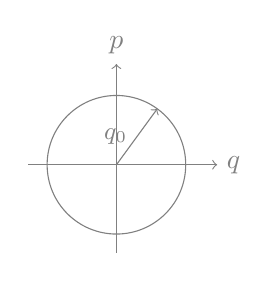
\begin{tikzpicture}[gray,scale=0.8]
  \draw[->] (-1.4,0) -- (1.6,0) node[right] {$q$};
  \draw[->] (0,-1.4) -- (0,1.6) node[above] {$p$};
  \draw (0,0) circle (1.1);
  \draw[->] (0,0) -- (0.65,0.89) node[midway,left] {\small $q_0$};
\end{tikzpicture}
\end{minipage}
\begin{minipage}{0.33\textwidth}
mapování do $\mathbb{C}$:
\[
  a \equiv \frac{1}{\sqrt2}(q + ip) = a_0e^{-i\omega t}
\]
\end{minipage}

\noindent\rule{\linewidth}{0.3pt}

\underline{Kvantová mechanika}
\[
  H = \frac{p^2}{2m} + \frac{m\omega^2}{2}x^2
  \quad\Big(\overset{x\text{-repr.}}{=} -\frac{\hbar^2}{2m}\dv[2]{x} + \frac{m\omega^2}{2}x^2
  \ \Big|\ \overset{p\text{-repr.}}{=} \frac{1}{2m}p^2 - \frac{\hbar^2m\omega^2}{2}\dv[2]{p}\Big)
\]
opět přejdeme k bezrozm.: \quad (OVĚŘTE: $p = -i\pdv{q}$, \ $q = i\pdv{p}$)
\[
  \vzorec{H = \frac{\hbar\omega}{2}(p^2 + q^2)}
  \qquad
  \Big[\overset{q\text{-repr.}}{=} \frac{\hbar\omega}{2}\Big(-\pdv[2]{q} + q^2\Big)
  \ \Big|\ \overset{p\text{-repr.}}{=} \frac{\hbar\omega}{2}\Big(p^2 - \pdv[2]{p}\Big)\Big]
\]

Podobně jako v klasickém případě zavedeme:
\[
  \vzorec{\hat a = \tfrac{1}{\sqrt2}(\hat q + i\hat p)}
  \quad\longleftrightarrow\quad
  \begin{aligned}
    \hat q &= \tfrac{1}{\sqrt2}(\hat a + \hat a^\dagger) \\
    \hat p &= \tfrac{1}{i\sqrt2}(\hat a - \hat a^\dagger)
  \end{aligned}
  \qquad\text{navíc: } [\hat q,\hat p] = \tfrac{1}{\hbar}[\hat X,\hat P] = i
\]
\[ \to\quad \hat a^\dagger = \tfrac{1}{\sqrt2}(\hat q - i\hat p) \]

\subsubsection*{VLASTNÍ VEKTORY $H$}
pozn: připomenout $\to$ stacionární stavy; význam pro měření $E$

Lze řešit přímo \pozn{přeškrtnuto: $\big[-\frac{\hbar^2}{2m}\dv[2]{x} + \frac{m\omega^2}{2}x^2\big]\psi(x) = E\psi(x)$, $q = x/x_0$} \\
\quad $\to$ \ $\dfrac{\hbar\omega}{2}\Big(-\pdv[2]{q} + q^2\Big)\psi(q) = E\psi(q)$ \\
\quad + asymptotika $q\to\infty$ ($q \gg \frac{2E}{\hbar\omega}$) \dots\ $\psi\sim e^{\pm q^2/2}$
+ hledání řeš.\ ve tvaru $p(q)e^{-q^2/2}$ \\
\hspace*{6cm} $\to$ UDĚLÁME JINAK

pozn: stejná rovnice vyjde v $p$-reprezentaci (srovn.\ klasické řešení)

%----------------------------------------------------------------------
\strana{QM-C-4}
\underline{nalezení spektra:}
\[
  [a,a^\dagger] = \tfrac12\big(-i[\hat q,\hat p] + i[\hat p,\hat q]\big) = 1
\]
\begin{definice}
$\hat N = \hat a^\dagger\hat a$ \quad \dots\ samosdružený operátor, fyz.\ význam?
\[
  \hat N = \tfrac12\big(\hat q^2 + \hat p^2 + i[\hat q,\hat p]\big) = \frac{\hat H}{\hbar\omega} - \frac12
  \qquad\text{tj.}\quad \vzorec{\hat H = \hbar\omega\big(\hat N + \tfrac12\big)}
\]
\end{definice}
tj.\ $[\hat H,\hat N] = 0$ \quad \dots\ spol.\ báze \quad \dots\ def.\ $\hat N\ket{n} = n\ket{n}$ \\
\quad potom \quad $\hat H\ket{n} = \hbar\omega\big(n + \frac12\big)\ket{n}$

\underline{spektrum $\hat N$?}

\begin{minipage}{0.68\textwidth}
důležité komut.\ relace \quad
$\begin{aligned}
  [\hat N,\hat a] &= \hat a^\dagger[a,a] + [a^\dagger,a]a = -a \\
  [N,a^\dagger] &= -\big([N,a]\big)^\dagger = a^\dagger
\end{aligned}$
\end{minipage}
\begin{minipage}{0.3\textwidth}
\fbox{$\begin{aligned} [N,a] &= -a \\ [N,a^\dagger] &= a^\dagger \end{aligned}$}
\end{minipage}

důsledek: \quad
$\begin{aligned}[t]
  Na^\dagger\ket{n} &= \big\{a^\dagger N + [N,a^\dagger]\big\}\ket{n} = (n+1)a^\dagger\ket{n} \\
  Na\ket{n} &= \big\{aN + [N,a]\big\}\ket{n} = (n-1)a\ket{n}
\end{aligned}$

\dots\ interpretace: \quad $a^\dagger, a$ \dots\ \kw{kreační, anihilační operátor}

normalizace: \quad $\mel{n}{a^\dagger a}{n} = n$ \quad $\to$ \quad $\vzorec{a\ket{n} = c\ket{n-1} = \sqrt n\ket{n-1}}$ \\
\quad \pozor{pozor} $\to$ obsahuje fázovou konvenci, smíme volit jen fázi $\ket{0}$, ostatní fixované

podob.: \quad $\mel{n}{aa^\dagger}{n} = \mel{n}{a^\dagger a + [a,a^\dagger]}{n} = (n+1)$ \quad
$\to$ \quad $\vzorec{a^\dagger\ket{n} = \sqrt{n+1}\ket{n+1}}$

s každou vl.\ hodnotou $n$ spektrum obsahuje $n\pm1, n\pm2, \dots$ \\
\quad + $N$ je \underline{pozitivně definitní}: $\mel{\psi}{a^\dagger a}{\psi} = \|a\psi\|^2 \geq 0$ \dots\ nelze sestupovat nekonečně dolů \\
\quad $\to$ nejnižší vl.\ č.: $n = 0$: \quad $a\ket{0} = 0$ \quad \dots\ tj.\ $\sigma = \{n = 0,1,2,\dots\}$
\begin{itemize}[nosep]
  \item vlastní čísla $\nearrow$
  \item formálně i vlastní vektory! \quad $\vzorec{\ket{n} = \frac{(a^\dagger)^n}{\sqrt{n!}}\ket{0}}$
\end{itemize}

Vlastní vektory v $x$ repr.\ (nebo $p$) neznáme, ale umíme počítat maticové elementy operátorů:
\[
  \hat x = \sqrt{\frac{\hbar}{2m\omega}}\,(a + a^\dagger) \qquad
  \hat P = i\sqrt{\frac{m\hbar\omega}{2}}\,(a^\dagger - a)
\]
\pozn{$\sqrt{\frac{\hbar}{2m\omega}} = \frac{x_0}{\sqrt2}$, \quad $\sqrt{\frac{m\hbar\omega}{2}} = \frac{\hbar}{x_0\sqrt2}$}

přitom: \quad $\mel{n'}{a}{n} = \sqrt n\,\delta_{n',n-1}$ \hfill $\mel{n'}{a^\dagger}{n} = \sqrt{n+1}\,\delta_{n',n+1}$

{\color{gray}
\[
  a = \begin{array}{c|cccc}
       & 0 & 1 & 2 & \cdots \\ \hline
     0 & 0 & \sqrt1 & 0 & \\
     1 & 0 & 0 & \sqrt2 & \\
     2 & 0 & 0 & 0 & \sqrt3 \\
     \vdots & & & & \ddots
  \end{array}
  \ (\text{sloupce } n,\ \text{řádky } n')
  \qquad\qquad
  a^\dagger = \begin{pmatrix}
     0 & & & \\
     \sqrt1 & 0 & & \\
     & \sqrt2 & 0 & \\
     & & \sqrt3 & \ddots
  \end{pmatrix}
\]}

%----------------------------------------------------------------------
\strana{QM-C-5}
\[
  \to\quad \mel{n'}{x}{n} = \frac{x_0}{\sqrt2}\begin{pmatrix} 0 & \sqrt1 & & \\ \sqrt1 & 0 & \sqrt2 & \\ & \sqrt2 & \ddots & \ddots \\ & & \ddots & \end{pmatrix}
  \qquad
  \mel{n'}{p}{n} = \frac{i\hbar}{x_0\sqrt2}\begin{pmatrix} 0 & \sqrt1 & & \\ -\sqrt1 & 0 & \sqrt2 & \\ & -\sqrt2 & \ddots & \ddots \\ & & \ddots & \end{pmatrix}
\]
$\to$ každý operátor $f(p,q)$ lze vyjádřit pomocí $a, a^\dagger$

\underline{\kw{vlnová funkce v $x$-reprezentaci}:}

$a\ket{0} = 0$ \quad \dots\ $\psi(x) = \braket{x}{0}$ \quad \dots\ $\psi(x) = \phi\big(q = \frac{x}{x_0}\big)$ \\
\quad $\hookrightarrow$ \ $(q + ip)\phi(q) = \Big(q + \dv{q}\Big)\phi(q) = 0$ \quad $\to$ \underline{řešení} \ $\phi_0(q) = Ne^{-\frac12q^2}$
\[
  \text{tj.}\quad \vzorec{\psi_0(x) = \frac{1}{\sqrt[4]{\pi x_0^2}}\,e^{-\frac12(x/x_0)^2}}
  \quad\longleftarrow\quad \int e^{-(x/x_0)^2}\dd x = x_0\sqrt\pi = \braket{\phi_0}{\phi_0} \ \ \text{(normování)}
\]

\underline{excitované stavy:} \quad
$a^\dagger = \frac{1}{\sqrt2}(q - ip) = \frac{1}{\sqrt2}\Big(\frac{x}{x_0} - \frac{ix_0}{\hbar}(-i\hbar)\dv{x}\Big) = \frac{1}{x_0\sqrt2}\Big(x - x_0^2\dv{x}\Big)$
\[
  \to\quad \psi_n(x) \equiv \braket{x}{n} = \frac{\mel{x}{(a^\dagger)^n}{0}}{\sqrt{n!}}
  = \frac{1}{\sqrt[4]\pi}\frac{1}{\sqrt{2^nn!}}\frac{1}{x_0^{n+\frac12}}\Big[x - x_0^2\dv{x}\Big]^ne^{-\frac12(x/x_0)^2}
\]
\[
  \text{nebo}\quad \vzorec{\psi_n(x) = \sqrt{\frac{1}{\sqrt\pi\,x_0\,n!\,2^n}}\;H_n(x/x_0)\,e^{-\frac12(x/x_0)^2}} \qquad (*)
\]
kde \quad $H_n(q) \equiv e^{q^2/2}\Big[q - \dv{q}\Big]^ne^{-q^2/2}$ \quad \dots\ \kw{Hermitův polynom}

\underline{pozn:}
\begin{itemize}
  \item Hermitovy polynomy jako OG-poly s vahou $w(x) = e^{-x^2}$ \\
        $\to$ \ $\int H_n(q)H_{n'}(q)w(q)\,\dd q = 0$ \quad \dots\ obecná teorie OG-poly $\to$ Gaussova kvadratura \\
        \pozn{Gram-Schmidt ortogonalizace monomů}
  \item ortogonální polynomy obecně splňují rekurentní relace, které získáme násobením $\hat x$: \\
        $\to$ v energetické reprezentaci:
        \[
          \mel{x}{\hat x}{n} = x\psi_n(x) = \frac{x_0}{\sqrt2}\big(\mel{x}{a}{n} + \mel{x}{a^\dagger}{n}\big)
          = \frac{x_0}{\sqrt2}\big(\sqrt n\,\psi_{n-1}(x) + \sqrt{n+1}\,\psi_{n+1}(x)\big)
        \]
        + dosazení $(*)$: \pozn{faktor $\frac{1}{\sqrt{2^nn!}}$} \quad
        $\dfrac{x}{x_0}H_n\Big(\dfrac{x}{x_0}\Big) = nH_{n-1}\Big(\dfrac{x}{x_0}\Big) + \dfrac12H_{n+1}\Big(\dfrac{x}{x_0}\Big)$
  \item pozn: velmi obecný systém \dots\ model stavů poblíž minima \\
        $\leftrightarrow$ izomorfní s mnoha částicemi v 1hladinovém systému \\
        \dots\ spektrum $= N\epsilon_0$ \quad \dots\ bosony (později)
  \item pozn: \pozn{vytvářející funkce: $e^{\xi^2 - (\xi-\eta)^2}$ \dots\
        $H_n(\xi) = \dv[n]{\eta}e^{\xi^2-(\xi-\eta)^2}\Big|_{\eta=0}$ \quad
        $\to\ = \sum_{n=0}^\infty\frac{H_n(\xi)}{n!}\eta^n$}
\end{itemize}

%----------------------------------------------------------------------
\strana{QM-C-6}
\subsection{Obecné vlastnosti stacionárních stavů částice v 1D skalárním potenciálu}
\[
  H\psi = E\psi \quad\xrightarrow[x\text{-repr.}]{}\quad
  \vzorec{-\frac{\hbar^2}{2m}\psi'' + V(x)\psi(x) = E\psi(x)} \qquad (*)
\]

\underline{OBECNĚ:} $\bullet$ \ OBYČEJNÁ LINEÁRNÍ DIF.\ ROVNICE 2.\ ř.
\begin{itemize}[nosep]
  \item[$\to$] existují dvě lin.\ nezávislá řešení $\psi(x) = \phi_1(x), \phi_2(x)$
  \item[$\to$] Lineární nezávislost \dots\ def.\ \
        $W(x) = \begin{pmatrix}\phi_1(x) & \phi_2(x)\\ \phi_1'(x) & \phi_2'(x)\end{pmatrix}$ \\
        $\Leftrightarrow \det W \neq 0$ \quad přitom \quad $\dv{x}|W| = \phi_1\phi_2'' - \phi_2\phi_1'' = 0$ \quad \pozn{dosazení za $\phi''$}
  \item[$\to$] obecné řešení $(*)$: \quad
        $\begin{pmatrix}\psi(x)\\ \psi'(x)\end{pmatrix} = W(x)\cdot A$; \quad
        $A = \begin{pmatrix}A_1\\ A_2\end{pmatrix}$ \dots\ vektor koeficientů
\end{itemize}

\begin{itemize}
  \item Nespojitosti potenciálu -- \kw{napojování řešení}:
  \begin{itemize}[nosep]
    \item[$\to$] vlnová funkce musí být spojitá -- jinak generuje členy $\delta'(x)$ v potenciálu
    \item[$\to$] derivace $\psi'(x)$ musí být spojitá -- jinak členy $\delta(x)$ v potenciálu
  \end{itemize}
  pozn: někdy se toho využívá a konstruují se modelové systémy s $\delta$-funkčním potenciálem \\
  \quad $V(x) = \underbrace{v(x)}_{\text{regulární člen}} + \lambda\delta(x - x_0)$
  \[
    \text{potom:}\quad \psi'(x_0+\varepsilon) - \psi'(x_0-\varepsilon) \equiv \Delta\psi' = \int_{x_0-\varepsilon}^{x_0+\varepsilon}\psi''\,\dd x
    \overset{(*)}{=} \frac{2m}{\hbar^2}\int_{x_0-\varepsilon}^{x_0+\varepsilon}\big[-E + v(x) + \lambda\delta(x - x_0)\big]\psi(x)\,\dd x
  \]
  \[ \text{tj.}\quad \vzorec{\Delta\psi' = \frac{2m}{\hbar^2}\lambda\,\psi(x_0)} \]
  $\to$ v bodech, kde je nanejvýš nespojitost typu skoku, tj.\ $\psi,\psi'$ spojité, \\
  můžeme podmínky napojování psát: \quad
  $\begin{pmatrix}\psi(x_0)\\ \psi'(x_0)\end{pmatrix} = W_-\cdot A_- = W_+A_+$ \\
  kde $W_\pm$ jsou matice Wronskiánu pod a nad bodem $x_0$ \\
  a $A_\pm = \begin{pmatrix}A_1^\pm\\ A_2^\pm\end{pmatrix}$ jsou koeficienty rozvoje řešení \dots\ pokud známe \\
  $A_+$, můžeme dopočíst $A_-$ a naopak \dots\ 2 rovnice, dvě neznámé (regulární \dots\ $\det W\neq0$)

  $\to$ lze redukovat na jednu rovnici \dots\ spojitost $\psi'/\psi = \dv{x}\ln\psi$ \\
  \dots\ \kw{Logaritmická derivace} \quad \dots\ důležitý jen poměr $A_1/A_2$ \quad (zbytek = normování)
  \item z poznámek výše: možno zkonstruovat dvě globální LNZ řešení \dots\ zbytek \dots\ okraj.\ podmínky
\end{itemize}

%----------------------------------------------------------------------
\strana{QM-C-7}
\begin{itemize}
  \item \kw{okrajové podmínky}

  napišme $(*)$ jako: \quad $\dfrac{\psi''}{\psi} = -\dfrac{2m}{\hbar^2}\big(E - V(x)\big)$
  \ $= \Big(-\dfrac{p(x)^2}{\hbar^2}\Big)$ \quad \dots\ znaménko \\
  $\to$ terminologie z klas.\ fyziky: body obratu, klasicky povolená/zakázaná oblast

  $\to$ obvyklý případ: $V(|x|\to\infty)\to$ konst \dots\ bůno $= 0$ \quad (fázová konvence/volba počátku $E$)

  \underline{pro $E < 0$:} dvě lnz.\ řešení: \quad $\psi = Ae^{\varkappa x} + Be^{-\varkappa x}$ \quad $x\to\infty$, \quad
  $\varkappa = \sqrt{\frac{2m}{\hbar^2}|E - V|}$ \\
  \quad (konst.\ pot $V = 0$) \quad \dots\ vyhovuje jen $A = 0$ $\uparrow$ \qquad $B = 0$ pro $x\to-\infty$

  pozn: dá se DK silnější tvrzení (Formánkova učebnice): \\
  \quad pokud $\frac{2m}{\hbar^2}(V - E) \geq \varkappa^2$ pro $x\geq a$, pak $\exists$ řešení
  $\psi_1 \geq Ae^{\varkappa x}$ a $\psi_2 \leq Be^{-\varkappa x}$ \\
  \quad \pozn{stručně princip důkazu \dots}

  \underline{pro $E > 0$:} dvě lnz.\ řešení: \quad
  $\psi = A\underbrace{e^{ikx}}_{\text{částice}\to} + B\underbrace{e^{-ikx}}_{\text{částice}\leftarrow}$ \quad $x\to\pm\infty$, \quad
  $k^2 = \frac{2m}{\hbar^2}(E - V) = p^2/\hbar^2$ \\
  \quad $\to$ srovn.\ s volnou částicí

  pozn: opět se dá DK silnější (Formánek): \\
  \quad pokud $\frac{2m}{\hbar^2}\big(E - V(x)\big) = k^2 + \Delta(x) \xrightarrow{x\to\infty} k^2$, \quad
  kde $\lim_{x\to\infty}x^\alpha\Delta(x) = 0$ pro nějaké $\alpha > 1$ \\
  \quad pak $\exists$ dvě lnz řešení $\sin(kx + \delta)$ a $\cos(kx + \delta)$ \\
  \quad \pozn{$\to$ princip -- fázová rovnice -- konverguje ke konst.}
\end{itemize}

\begin{minipage}{0.68\textwidth}
$\to$ shrnutí \dots\ \kw{kvantová jáma} (potenciálová) (angl.\ studna = well) \\
\pozn{celé $V > 0$ neobsahuje případ $E < 0$}
\end{minipage}
\begin{minipage}{0.3\textwidth}
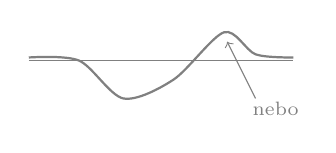
\begin{tikzpicture}[gray,scale=0.8]
  \draw[thin] (-2,0) -- (2.2,0);
  \draw[thick] plot[smooth] coordinates {(-2,0.05) (-1.2,0) (-0.5,-0.6) (0.3,-0.3) (1.1,0.45) (1.6,0.1) (2.2,0.05)};
  \draw[->] (1.6,-0.6) -- (1.15,0.3);
  \node[below right] at (1.4,-0.5) {\scriptsize nebo};
\end{tikzpicture}
\end{minipage}

klasická částice $\to$ povolené energie $E > V_0 = \min V(x)$ \\
\hspace*{3.2cm} $\to$ pro $E < 0$ \dots\ vázané stavy \\
\hspace*{3.2cm} $\to$ pro $E > 0$ \dots\ rozptylové (nebo za bariérou chycené)

kvantová částice:
\begin{veta}[Vázané stavy]
\fbox{$E < 0$} $\to$ \kw{vázané stavy} \dots\ $\psi\in L^2$, ale obě okrajové podmínky
($A = 0$ v $\infty$, $B = 0$ v $-\infty$) \\
lze splnit jen pro diskrétní $E = E_B$ \\
navíc \quad $E_B = \langle H\rangle = \underbrace{\langle T\rangle}_{\geq0} + \underbrace{\langle V\rangle}_{\geq V_0} \geq V_0$
\quad \dots\ tj.\ $E_B\in\langle V_0, 0)$
\end{veta}

\begin{veta}[Oscilační věta]
dk.\ rozborem chování $\frac{\psi''}{\psi} = -\frac{p^2(x)}{\hbar^2}$ \pozn{nesnadné}

$E_0 < E_1 < E_2 \dots$ energie váz.\ stavů \dots\ $\ket{\psi_\nu}$; $\nu = 0,1,2,\dots$ přísl.\ stavy \\
potom $\psi_\nu(x)$ má právě $\nu$ nulových bodů $\psi_\nu(x_0) = 0$ \\
a navíc mezi $\forall$ dvěma nul.\ body $\psi_\nu$ leží nulový bod $\psi_{\nu+1}$
\end{veta}
pozn: \dots\ semiklasický pohled $\hbar$ \dots\ plocha v $px$-prostoru \\
pozn: pokud $V(x) < 0\ \forall x$ \dots\ dá se dk, že $\exists$ alesp.\ jeden váz.\ stav (Var.\ princip)

%----------------------------------------------------------------------
\strana{QM-C-8}
\fbox{$E > 0$}
\begin{itemize}[nosep]
  \item[$\to$] jen zobecněné vl.\ stavy $\psi(x)$ omezená fce \\
        pro $\forall$ energii $E$ existují dva stavy \dots\ klasifikujeme později $\to$ teorie rozptylu
\end{itemize}

\begin{center}
\begin{tikzpicture}[>=Stealth]
  \node[left,align=right] at (-0.3,0.3) {okraj.\ podm.: \\ {\small lze DK, že jsou} \\ {\small ortogonální} $\to$};
  % levý box: částice nalétá zleva
  \draw (0,-0.6) rectangle (5,1.2);
  \node at (1.2,0.85) {$e^{ikx} + Re^{-ikx}$};
  \node at (3.9,0.85) {$Te^{ikx}$};
  \draw[->] (0.6,0.4) -- (1.6,0.4) arc (90:-90:0.12) -- (0.8,0.16);
  \draw[->] (3.4,0.35) -- (4.3,0.35);
  \node at (2.5,-0.3) {částice nalétá zleva};
  % pravý box: částice nalétá zprava
  \draw (5.3,-0.6) rectangle (10.3,1.2);
  \node at (6.2,0.85) {$Te^{-ikx}$};
  \node at (8.9,0.85) {$e^{-ikx} + Re^{ikx}$};
  \draw[->] (6.6,0.35) -- (5.7,0.35);
  \draw[->] (9.5,0.4) -- (8.5,0.4) arc (90:270:0.12) -- (9.3,0.16);
  \node at (7.8,-0.3) {částice nalétá zprava};
\end{tikzpicture}
\end{center}

$\to$ v případě symetrického potenciálu $V(x) = V(-x)$ \\
\quad tj.\ $[\mathcal{P},V] = 0$, \ $\mathcal{P}$ \dots\ parita, lze volit řešení s paritou $\lambda = \pm1$ \\
\hspace*{5cm} \dots\ $\psi(|x|\to\infty)\to\cos(k|x| + \delta), \ \pm\sin(k|x| + \delta)$ \\
pozn: $\hookrightarrow$ pro váz.\ stavy platí $\psi_\nu(-x) = (-1)^\nu\psi(x)$ \quad (srovn.\ oscilační věta)

$\to$ to, že $V(x)\in\mathbb{R}$, implikuje, že pokud $\psi$ řeší $(*)$, pak $\psi^*$ řeší \\
\quad tj.\ také $\frac12(\psi + \psi^*) = \mathrm{Re}\,\psi$ a $\frac{1}{2i}(\psi - \psi^*) = \mathrm{Im}\,\psi$ řeší $(*)$ \\
\quad \dots\ lze vždy vybrat reál.\ řešení \quad \pozn{zmínit se o $\mathrm{Im}\,V\neq0$ -- otevřené systémy}

\fbox{$V_{+\infty}\neq V_{-\infty}$} \dots\ hodí se jako model:
\begin{itemize}[nosep]
  \item[] $E < \min(V_+,V_-)$ \dots\ váz.\ stavy
  \item[] $\min(V_\pm) < E < \max(V_+,V_-)$ \dots\ $\forall E$ existuje jeden stav \dots\ kontinuum
  \item[] $E > \max(V_+,V_-)$ \dots\ dvě kontinua
\end{itemize}
pozn: v klas.\ fyzice \dots\ stavy v kontinuu (trapping) \\
\phantom{pozn:} v kvant.\ fyzice \dots\ není díky tunelování, ale později \dots\ rezonance

\fbox{$V = \infty$} \dots\ někdy je užitečný model \\
\quad \dots\ dá se chápat jako $\lim V\to\infty$ \\
\quad vyjde \dots\ $\psi = 0$ v oblasti, kde $V = \infty$ \\
\quad\quad $\psi'$ nemusí být spojitá na hranici oblasti \quad + pozn $\blacktriangle$ \dots\ na druhé str.

\subsection*{PŘESNĚ ŘEŠITELNÉ MODELY}
\begin{itemize}
  \item napojování a $\delta$-potenciály (včetně $V = \infty$)
  \item konst.\ potenciál, Lineární pot.\ a LHO (obecné řeš.\ definují spec.\ fci)
  \item \kw{Woods--Saxon} \quad $V(x) = -\dfrac{V_0}{1 + e^{\alpha x}}$ \quad $\psi$ \dots\ Hypergeometrická funkce

  \begin{minipage}{0.45\textwidth}
  \begin{tikzpicture}[gray,scale=0.9]
    \draw[thick,domain=-3:3,samples=60] plot (\x,{1.4/(1+exp(-2.5*\x))});
    \node[left] at (-3,0) {$-V_0$};
    \node[right] at (3,1.4) {$V = 0$};
  \end{tikzpicture}
  \end{minipage}
  \begin{minipage}{0.5\textwidth}
  pro $E > 0$:
  \[
    |R(E)|^2 = \frac{\sinh^2\big(\pi(k - k')/\alpha\big)}{\sinh^2\big(\pi(k + k')/\alpha\big)}
  \]
  \end{minipage}

  \kw{kvantový odraz} (nemá klas.\ obdobu)
\end{itemize}

%----------------------------------------------------------------------
\strana{QM-C-9}
\begin{itemize}
  \item pot.\ jáma a bariéra \quad $V(x) = \pm V_0\cosh(\alpha x)$ \quad \dots\ spec.\ fce.
  \item \kw{Morseho potenciál}: \quad $V(x) = D\big(e^{-2a(x-x_0)} - 2e^{-a(x-x_0)}\big)$

  \begin{minipage}{0.6\textwidth}
  váz.\ stavy: \quad $E_\nu = -\big(\lambda - n - \tfrac12\big)^2\cdot\dfrac{a^2\hbar^2}{2m}$ \\[4pt]
  \hspace*{2.2cm} $\lambda = \dfrac{1}{a\hbar}\sqrt{2mD}$

  \medskip
  $\psi_n$ \dots\ dá se vyjádřit pomocí Laguerre poly.
  \end{minipage}
  \begin{minipage}{0.35\textwidth}
  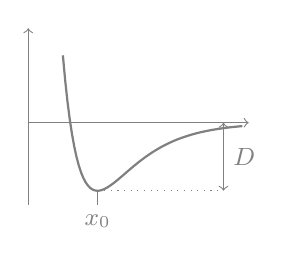
\begin{tikzpicture}[gray,scale=0.8]
    \draw[->] (0,-1.3) -- (0,1.5);
    \draw[->] (0,0) -- (3.5,0);
    \draw[thick,domain=0.55:3.4,samples=80] plot (\x,{1.2*(exp(-2*1.6*(\x-1.1)) - 2*exp(-1.6*(\x-1.1)))*0.9});
    \draw[thin] (1.1,-1.08) -- (1.1,-1.3) node[below] {\small $x_0$};
    \draw[<->] (3.1,0) -- (3.1,-1.08) node[midway,right] {\small $D$};
    \draw[dotted] (1.1,-1.08) -- (3.1,-1.08);
  \end{tikzpicture}
  \end{minipage}
\end{itemize}

\underline{pozn $\blacktriangle$:} (Ballentine) \\
v ošklivých potenciálech mohou existovat váz.\ st.\ v kont. \\
\quad př: \quad $V(r)\xrightarrow{r\to\infty}\dfrac{\sin(2kr)}{r}$ \quad a \quad
$\psi(r) = f(r)\dfrac{\sin kr}{kr}$, \quad $E = \frac12k^2$ \\
\quad \dots\ $\psi\in L^2$ a přitom $E > 0$ \quad \dots\ důvod: odrazy od bariér, \\
\hspace*{5cm} jejichž výška jde pomalu k $0$ pro $x\to\infty$

\underline{pozn:} v 1D se dá DK, že pro $V(x) < 0 = V_\infty$ $\exists$ alesp.\ jeden váz.\ stav. \\
\hspace*{3.5cm} $\hookrightarrow$ později z variač.\ principu

